\documentclass[12pt, a4paper]{article}

% ── Packages ──────────────────────────────────────────────────────────────────
\usepackage[a4paper, margin=2.5cm]{geometry}
\usepackage{graphicx}
\usepackage{float}
\usepackage{amsmath}
\usepackage{amssymb}
\usepackage{xcolor}
\usepackage{mdframed}
\usepackage{parskip}
\usepackage{enumitem}
\usepackage{titlesec}
\usepackage{booktabs}
\usepackage{hyperref}
\usepackage[T1]{fontenc}
\usepackage{tikz}
\usetikzlibrary{arrows.meta}

% ── Graphics path ─────────────────────────────────────────────────────────────
\graphicspath{{../../Images_for_latex/Lecture_4/}}

% ── Colours ───────────────────────────────────────────────────────────────────
\definecolor{keyblue}{RGB}{30, 80, 160}
\definecolor{keybluebg}{RGB}{220, 235, 255}
\definecolor{noteorange}{RGB}{200, 100, 0}
\definecolor{noteorangebg}{RGB}{255, 240, 215}
\definecolor{warnred}{RGB}{180, 30, 30}
\definecolor{warnredbg}{RGB}{255, 220, 220}
\definecolor{defgreen}{RGB}{20, 110, 50}
\definecolor{defgreenbg}{RGB}{215, 245, 225}
\definecolor{headernavy}{RGB}{25, 35, 90}

% ── Box environments ──────────────────────────────────────────────────────────
\newmdenv[linecolor=keyblue,backgroundcolor=keybluebg,linewidth=1.5pt,
  leftline=true,rightline=false,topline=false,bottomline=false,
  innerleftmargin=10pt,innerrightmargin=8pt,
  innertopmargin=6pt,innerbottommargin=6pt,
  skipabove=8pt,skipbelow=8pt]{keybox}

\newmdenv[linecolor=noteorange,backgroundcolor=noteorangebg,linewidth=1.5pt,
  leftline=true,rightline=false,topline=false,bottomline=false,
  innerleftmargin=10pt,innerrightmargin=8pt,
  innertopmargin=6pt,innerbottommargin=6pt,
  skipabove=8pt,skipbelow=8pt]{notebox}

\newmdenv[linecolor=warnred,backgroundcolor=warnredbg,linewidth=1.5pt,
  leftline=true,rightline=false,topline=false,bottomline=false,
  innerleftmargin=10pt,innerrightmargin=8pt,
  innertopmargin=6pt,innerbottommargin=6pt,
  skipabove=8pt,skipbelow=8pt]{warnbox}

\newmdenv[linecolor=defgreen,backgroundcolor=defgreenbg,linewidth=1.5pt,
  leftline=true,rightline=false,topline=false,bottomline=false,
  innerleftmargin=10pt,innerrightmargin=8pt,
  innertopmargin=6pt,innerbottommargin=6pt,
  skipabove=8pt,skipbelow=8pt]{defbox}

% ── Section formatting ────────────────────────────────────────────────────────
\titleformat{\section}[block]{\large\bfseries\color{headernavy}}{}{0pt}{}
  [\vspace{2pt}\rule{\linewidth}{0.8pt}\vspace{4pt}]
\titleformat{\subsection}[block]{\normalsize\bfseries\color{keyblue}}{}{0pt}{}

% ── Document ──────────────────────────────────────────────────────────────────
\begin{document}

\begin{center}
  {\LARGE\bfseries\color{headernavy} Sensors \& Systems}\\[4pt]
  {\large Kalman Filter for Nonlinear Systems --- EKF \& UKF}\\[2pt]
  {\normalsize Torben Knudsen \quad|\quad Electronic Systems, 8th Semester}
\end{center}

\vspace{4pt}\hrule height 1.2pt\vspace{12pt}

% ==============================================================================
\section*{Section 1 \quad Why the Standard KF Breaks for Nonlinear Systems}
% ==============================================================================

The standard Kalman filter from Lecture~3 is the optimal estimator
for \emph{linear} systems.
Most real physical systems, however, are \textbf{nonlinear} to some
degree --- a pendulum, a robot arm, a drone, a chemical reactor.
This raises three important questions:

\begin{itemize}[leftmargin=1.4em]
  \item Can states still be estimated in nonlinear systems?
  \item Does an \emph{optimal} estimator exist?
  \item Does a \emph{good} (not necessarily optimal) estimator exist?
\end{itemize}

The short answers: yes, sometimes, and yes.
An optimal closed-form estimator generally does \emph{not} exist for
nonlinear systems --- but practical approximations (EKF and UKF)
work well in most cases.

% ------------------------------------------------------------------------------
\subsection*{What does ``nonlinear'' actually mean here?}
% ------------------------------------------------------------------------------

In the linear KF the state equation and measurement equation use
\emph{matrices}:
\[
  x_{k+1} = \Phi_k x_k + \Gamma_k u_k + w_k, \qquad
  y_k     = H_k x_k + D_k u_k + v_k
\]
A matrix multiplication $\Phi_k x_k$ is \textbf{linear}: the output
scales proportionally with the input.
Formally, a function $f$ is linear if:
\begin{itemize}[leftmargin=1.4em, topsep=2pt]
  \item Double the input $\Rightarrow$ double the output:
        $f(2x) = 2f(x)$
  \item Add two inputs $\Rightarrow$ add the outputs:
        $f(x+y) = f(x) + f(y)$
\end{itemize}
A matrix satisfies both --- it only stretches, rotates, or flips a
vector, never bends or curves it.
This means the KF can compute exact means and covariances because
everything stays predictable and proportional.

In a nonlinear system the matrices $\Phi_k$ and $H_k$ are replaced
by arbitrary \textbf{functions} $f$ and $h$:
\[
  x_{k+1} = f(x_k,\, u_k) + w_k, \qquad
  y_k     = h(x_k,\, u_k) + v_k
\]
$f$ and $h$ can be anything --- $\sin$, $\cos$, products of states,
square roots.
A nonlinear function breaks the linearity rules:
$\sin(2x) \neq 2\sin(x)$, so the output no longer scales
predictably.
The noise assumptions are unchanged ($w_k$ and $v_k$ white and
uncorrelated), but the functions themselves can bend and curve.

\begin{notebox}
  \textbf{Concrete examples of nonlinear $f$ and $h$.}
  \begin{itemize}[leftmargin=1.4em, topsep=2pt]
    \item \textbf{Pendulum}: the state is angle $\theta$ and angular
          velocity $\dot\theta$.
          The state equation contains $\sin\theta$ ---
          nonlinear in the state.
    \item \textbf{Range sensor}: you measure the distance to an
          object whose position $(p_x, p_y)$ is the state.
          $h = \sqrt{(p_x - s_x)^2 + (p_y - s_y)^2}$ --- a square
          root of states, nonlinear.
    \item \textbf{IMU attitude} (from Lecture~5): converting gyro
          rates to orientation involves $\sin$ and $\cos$ of the
          current roll/pitch/yaw angles --- nonlinear.
  \end{itemize}
\end{notebox}

% ------------------------------------------------------------------------------
\subsection*{The NL DD estimation problem}
% ------------------------------------------------------------------------------

The discrete-discrete nonlinear problem has the same structure as
the linear DD problem --- it just uses $f$ and $h$ instead of
matrices:

\[
  x_{k+1} = f(x_k,\, u_k) + w_k, \quad w_k \sim \mathrm{NID}(0,\, Q_k)
\]
\[
  y_k = h(x_k,\, u_k) + v_k, \quad v_k \sim \mathrm{NID}(0,\, R_k)
\]
\[
  E\!\left[w_k\, v_l^\top\right] = 0
\]

\begin{center}
\renewcommand{\arraystretch}{1.4}
\begin{tabular}{p{1.8cm} p{3.2cm} p{7.5cm}}
  \toprule
  \textbf{Symbol} & \textbf{Name} & \textbf{Meaning} \\
  \midrule
  $x_k$   & State vector        & What we want to estimate (position, velocity, angle, \ldots) \\
  $f(\cdot,\cdot)$ & State function & Nonlinear function describing how the state evolves; \textbf{replaces} $\Phi_k$ from the linear KF \\
  $u_k$   & Input/control       & Known input applied at step $k$ (force, voltage, \ldots) \\
  $w_k$   & Process noise       & Random disturbances; $w_k \sim \mathrm{NID}(0,\,Q_k)$ \\
  $Q_k$   & Process noise cov.  & Covariance of $w_k$ --- how uncertain the state equation is \\
  \midrule
  $y_k$   & Measurement vector  & What the sensor actually outputs at step $k$ \\
  $h(\cdot,\cdot)$ & Measurement function & Nonlinear function mapping state to sensor output; \textbf{replaces} $H_k$ from the linear KF \\
  $v_k$   & Measurement noise   & Sensor noise; $v_k \sim \mathrm{NID}(0,\,R_k)$ \\
  $R_k$   & Meas.\ noise cov.   & Covariance of $v_k$ --- how noisy the sensor is \\
  \bottomrule
\end{tabular}
\end{center}

Given all measurements up to step $k$:
\[
  \mathcal{Y}_k \triangleq y_0, y_1, \ldots y_k,\quad
  u_0, u_1, \ldots u_k, \quad
  x_0 \sim \mathcal{N}(\hat{x}_0,\, P_0)
\]

\begin{notebox}
  $\mathcal{Y}_k$ is everything the filter is \textbf{allowed to use} ---
  its full information set:
  \begin{itemize}[leftmargin=1.4em, topsep=2pt]
    \item $y_0, y_1, \ldots y_k$ --- every sensor reading collected so far.
    \item $u_0, u_1, \ldots u_k$ --- every input/control signal applied
          (known exactly, because \emph{you} applied them).
    \item $x_0 \sim \mathcal{N}(\hat{x}_0,\, P_0)$ --- the initial guess
          for the starting state: modelled as Gaussian with mean
          $\hat{x}_0$ and covariance $P_0$.
  \end{itemize}
  The hat $\,\hat{\cdot}\,$ always denotes an \textbf{estimate}:
  $\hat{x}_k$ is our best guess for the true state $x_k$.
\end{notebox}

Find $\hat{x}_k$ that minimises the mean square error:
\[
  E\!\left[(x_k - \hat{x}_k)^\top M (x_k - \hat{x}_k)\right], \quad M \geq 0
\]

\begin{notebox}
  \textbf{What is $M$?}\\
  $M$ is a \textbf{weighting matrix} --- it controls how much the cost
  function penalises errors in each component of the state.
  The expression $(x_k - \hat{x}_k)^\top M\,(x_k - \hat{x}_k)$ is a
  weighted sum of squared errors between the true state and the estimate.\\[4pt]
  The key insight: the condition is only $M \geq 0$ (any valid weighting).
  This means \textbf{no matter how you weight the errors, the same
  estimator wins} --- the conditional mean $E[x_k \mid \mathcal{Y}_k]$.
  You cannot do better in any direction simultaneously, regardless of
  whether you care more about position error, velocity error, or any
  combination.
  This is the theoretical justification for why the KF (which tracks
  the conditional mean) is the optimal estimator for linear Gaussian
  systems.
\end{notebox}

\begin{center}
\renewcommand{\arraystretch}{1.5}
\begin{tabular}{p{2cm} p{6cm} p{6cm}}
  \toprule
  & \textbf{Linear DD (Lecture 3)} & \textbf{Nonlinear DD} \\
  \midrule
  State eq. &
    $x_{k+1} = \Phi_k x_k + \Gamma_k u_k + w_k$ &
    $x_{k+1} = f(x_k, u_k) + w_k$ \\
  Meas. eq. &
    $y_k = H_k x_k + D_k u_k + v_k$ &
    $y_k = h(x_k, u_k) + v_k$ \\
  Optimal estimator &
    Kalman filter --- exact, closed form &
    No closed-form solution in general \\
  Practical estimator &
    KF &
    EKF or UKF \\
  \bottomrule
\end{tabular}
\end{center}

% ------------------------------------------------------------------------------
\subsection*{The NL CD estimation problem}
% ------------------------------------------------------------------------------

The continuous-discrete nonlinear problem follows the same extension:
replace the linear continuous model with a nonlinear SDE.
\[
  dx(t) = f\!\left(x(t),\, u(t)\right) dt + d\omega(t),
  \quad \omega(t) \sim \mathcal{W}(Q(t))
\]
\[
  y(t_k) = h\!\left(x(t_k),\, u(t_k)\right) + v_k,
  \quad v_k \sim \mathrm{NID}(0,\, R_k)
\]

\begin{center}
\renewcommand{\arraystretch}{1.4}
\begin{tabular}{p{1.8cm} p{3.2cm} p{7.5cm}}
  \toprule
  \textbf{Symbol} & \textbf{Name} & \textbf{Meaning} \\
  \midrule
  $x(t)$  & State vector        & Continuously evolving state (angle, concentration, \ldots) \\
  $f(\cdot,\cdot)$ & Drift function & Nonlinear function for how the state changes continuously; \textbf{replaces} $F(t)x + B(t)u$ from the linear CD model \\
  $u(t)$  & Continuous input    & Known control signal varying continuously in time \\
  $d\omega(t)$ & Wiener increment & Continuous process noise; infinitesimal random kick at each instant \\
  $Q(t)$  & Spectral density    & Intensity of the continuous noise $d\omega(t)$ \\
  \midrule
  $y(t_k)$ & Measurement        & Discrete sensor output, sampled at times $t_0, t_1, \ldots$ \\
  $h(\cdot,\cdot)$ & Meas.\ function & Nonlinear mapping from state to sensor reading; \textbf{replaces} $H_k$ \\
  $v_k$   & Measurement noise   & Discrete sensor noise; $v_k \sim \mathrm{NID}(0,\,R_k)$ \\
  $R_k$   & Meas.\ noise cov.   & Covariance of $v_k$ --- how noisy the sensor is \\
  \bottomrule
\end{tabular}
\end{center}

The continuous state evolves according to a \emph{nonlinear} SDE
between measurement times.
The measurement at each discrete sample $t_k$ is a nonlinear
function of the current state.

\begin{warnbox}
  \textbf{Why no optimal estimator exists for nonlinear systems.}\\
  In the linear case, the conditional distribution $p(x_k \mid
  \mathcal{Y}_k)$ is always Gaussian, and its mean and covariance
  are all you need --- the KF tracks them exactly.\\[4pt]
  For a nonlinear system, passing a Gaussian through a nonlinear
  function $f$ produces a distribution that is \emph{no longer
  Gaussian} --- it is bent, skewed, multi-modal.
  Tracking the full shape of that distribution exactly requires
  infinitely many parameters.\\[4pt]
  Both EKF and UKF sidestep this by forcing the distribution to
  stay Gaussian (approximating it by a mean and covariance), just
  computed differently:
  \begin{itemize}[leftmargin=1.4em, topsep=2pt]
    \item \textbf{EKF}: approximate $f$ as linear (tangent line at
          the current estimate) then propagate the Gaussian through
          that linear approximation.
    \item \textbf{UKF}: keep $f$ exact but approximate the output
          Gaussian using a small set of carefully chosen sample
          points (sigma points).
  \end{itemize}
\end{warnbox}

\begin{keybox}
  \textbf{Key takeaways --- Section 1}
  \begin{itemize}[leftmargin=1.4em, topsep=2pt]
    \item Nonlinear means the state/measurement functions are
          $f(x,u)$ and $h(x,u)$ --- arbitrary functions, not
          matrices.
    \item The noise assumptions are unchanged: white, Gaussian,
          uncorrelated.
    \item No optimal closed-form estimator exists for nonlinear
          systems --- passing a Gaussian through a nonlinear
          function destroys its Gaussian shape.
    \item EKF and UKF are both approximations that keep the
          distribution Gaussian, just with different strategies
          for computing the mean and covariance after the
          nonlinear step.
  \end{itemize}
\end{keybox}

Compare the linear and nonlinear forms side by side:
\begin{center}
\renewcommand{\arraystretch}{1.5}
\begin{tabular}{p{2cm} p{5.8cm} p{5.8cm}}
  \toprule
  & \textbf{Linear DD} & \textbf{Linear CD} \\
  \midrule
  State eq. &
    $x_{k+1} = \Phi_k x_k + \Gamma_k u_k + w_k$ &
    $dx(t) = F(t)x(t)\,dt + B(t)u(t)\,dt + d\omega(t)$ \\
  Meas. eq. &
    $y_k = H_k x_k + D_k u_k + v_k$ &
    $y(t_k) = H_k x(t_k) + D_k u(t_k) + v_k$ \\
  State noise &
    $w_k \sim \mathrm{NID}(0,\,Q_k)$ &
    $\omega(t) \sim \mathcal{W}(Q(t))$ \\
  Meas. noise &
    $v_k \sim \mathrm{NID}(0,\,R_k)$ &
    $v_k \sim \mathrm{NID}(0,\,R_k)$ \\
  \bottomrule
\end{tabular}
\end{center}

\begin{center}
\renewcommand{\arraystretch}{1.5}
\begin{tabular}{p{2cm} p{5.8cm} p{5.8cm}}
  \toprule
  & \textbf{NL DD} & \textbf{NL CD} \\
  \midrule
  State eq. &
    $x_{k+1} = f(x_k,\, u_k) + w_k$ &
    $dx(t) = f(x(t),\, u(t))\,dt + d\omega(t)$ \\
  Meas. eq. &
    $y_k = h(x_k,\, u_k) + v_k$ &
    $y(t_k) = h(x(t_k),\, u(t_k)) + v_k$ \\
  State noise &
    $w_k \sim \mathrm{NID}(0,\,Q_k)$ &
    $\omega(t) \sim \mathcal{W}(Q(t))$ \\
  Meas. noise &
    $v_k \sim \mathrm{NID}(0,\,R_k)$ &
    $v_k \sim \mathrm{NID}(0,\,R_k)$ \\
  \bottomrule
\end{tabular}
\end{center}

% ==============================================================================
\section*{Section 2 \quad The Extended Kalman Filter (EKF)}
% ==============================================================================

% ------------------------------------------------------------------------------
\subsection*{Basic idea}
% ------------------------------------------------------------------------------

The EKF keeps the same two-step structure as the standard KF
(time update + measurement update), but handles the nonlinear functions
$f$ and $h$ by \textbf{linearising} them around the current best
estimate before applying the KF equations.
Four key points from the slides:

\begin{itemize}[leftmargin=1.4em, topsep=2pt]
  \item The optimal estimator $E(x_k \mid \mathcal{Y}_k)$ cannot
        normally be obtained for nonlinear systems.
  \item The KF framework \emph{can} still be used if we first
        linearise the nonlinear system.
  \item Linearisation can be done with a \textbf{fixed} point
        (chosen once) or a \textbf{variable} point (updated every step).
  \item The best EKF uses the \textbf{most recent state estimate} as
        the linearisation point and keeps the nonlinear functions $f$
        and $h$ wherever they appear directly (not just their
        linearised versions).
\end{itemize}

% ------------------------------------------------------------------------------
\subsection*{Linearisation: the Jacobian matrices}
% ------------------------------------------------------------------------------

To linearise $f$ and $h$ with respect to the state $x$, we take their
\textbf{partial derivatives} --- these are called Jacobian matrices:

\[
  F_k(x) \triangleq \frac{\partial f(x)}{\partial x^\top}, \qquad
  H_k(x) \triangleq \frac{\partial h(x)}{\partial x^\top}
\]

\begin{center}
\renewcommand{\arraystretch}{1.4}
\begin{tabular}{p{1.8cm} p{3.2cm} p{7.5cm}}
  \toprule
  \textbf{Symbol} & \textbf{Name} & \textbf{Meaning} \\
  \midrule
  $F_k(x)$ & State Jacobian   & $n \times n$ matrix of partial derivatives of $f$; replaces $\Phi_k$ in the covariance equations \\
  $H_k(x)$ & Output Jacobian  & $p \times n$ matrix of partial derivatives of $h$; replaces $H_k$ in the gain and covariance equations \\
  \bottomrule
\end{tabular}
\end{center}

\begin{notebox}
  \textbf{What is a Jacobian?}\\
  For a nonlinear function $f: \mathbb{R}^n \to \mathbb{R}^n$, the
  Jacobian $\partial f / \partial x^\top$ is the matrix of all first
  partial derivatives --- entry $(i,j)$ is $\partial f_i / \partial x_j$.
  It is the best local \emph{linear approximation} to $f$ at a given
  point: a flat tangent plane that matches $f$'s slope at that point.\\[4pt]
  The argument $x$ passed to $F_k$ and $H_k$ should always be the
  \textbf{most recent estimate} of the state:
  use $\hat{x}_{k|k-1}$ for $H_k$ (before the measurement update)
  and $\hat{x}_{k|k}$ for $F_k$ (after the measurement update).
  This keeps the linearisation as accurate as possible.
\end{notebox}

\begin{notebox}
  \textbf{How linearisation actually works --- a 1D example.}\\[4pt]
  Say the state equation is $f(x) = \sin(x)$.
  That is nonlinear --- the KF cannot handle it directly.
  But zoom in close to any specific point and a curve looks like a
  straight line.
  Linearisation is just replacing the curve with the \textbf{tangent
  line} at the current best guess, via a Taylor expansion around
  $\hat{x}$:
  \[
    f(x) \approx \underbrace{f(\hat{x})}_{\text{(1)}}
                 + \underbrace{F_k}_{df/dx\,|_{\hat{x}}}
                   \underbrace{(x - \hat{x})}_{\text{(2)}}
  \]
  For $\sin(x)$ the slope is $\cos(\hat{x})$, so if
  $\hat{x} = 0.1$:
  \[
    \sin(x) \approx \sin(0.1) + \cos(0.1)\cdot(x - 0.1)
  \]
  That is a straight line --- the KF can work with that.\\[6pt]
  \textbf{The two parts play different roles in the EKF:}
  \begin{itemize}[leftmargin=1.4em, topsep=2pt]
    \item \textbf{Part (1) --- mean update.}
          $x$ \emph{is} replaced by the estimate:
          $\hat{x}_{k+1|k} = f(\hat{x}_{k|k}, u_k)$.
          Plug the best guess directly into the nonlinear function.
    \item \textbf{Part (2) --- covariance update.}
          $x$ here is the \emph{true} (unknown) state.
          The difference $(x - \hat{x})$ is the error.
          Propagating this error through the linearised function gives:
          \[
            (x_{k+1} - \hat{x}_{k+1|k})
            \approx F_k\,(x_k - \hat{x}_{k|k}) + w_k
          \]
          Square and take the expectation $\Rightarrow$ the error
          never appears explicitly; it disappears into the covariance:
          \[
            P_{k+1|k} = F_k\,P_{k|k}\,F_k^\top + Q_k
          \]
  \end{itemize}
  \textbf{Why the most recent estimate?}
  Because the tangent-line approximation is only accurate
  \emph{near} the expansion point.
  Using the most recent $\hat{x}_{k|k}$ puts the linearisation
  exactly where we think the true state is.
  A fixed expansion point chosen at the start would drift further
  and further from the truth as the state evolves.\\[4pt]
  $F_k$ and $H_k$ are \textbf{not constant} --- they are recomputed
  at every step by plugging the current state estimate into the
  derivative formula.
\end{notebox}

% ------------------------------------------------------------------------------
\subsection*{EKF algorithm for the nonlinear DD problem}
% ------------------------------------------------------------------------------

The EKF has the same two-step structure as the linear KF.
To see exactly what changed, each equation below is shown side by side
with its linear KF counterpart.

\textbf{Initial conditions:}
\[
  x_0 \sim \mathcal{N}(\hat{x}_{0|-1},\; P_{0|-1})
\]

% ── Step B ────────────────────────────────────────────────────────────────────
\textbf{Step B --- Measurement update} (after receiving $y_k$ and $u_k$):

\medskip
\begin{center}
\renewcommand{\arraystretch}{1.6}
\begin{tabular}{p{0.9cm} p{5.2cm} p{5.2cm}}
  \toprule
  & \textbf{Linear KF} & \textbf{EKF} \\
  \midrule
  $\hat{y}_{k|k-1}$ &
    $H_k \hat{x}_{k|k-1} + D_k u_k$ &
    $h(\hat{x}_{k|k-1},\, u_k)$ \\
  $\tilde{y}_{k|k-1}$ &
    $y_k - \hat{y}_{k|k-1}$ &
    $y_k - \hat{y}_{k|k-1}$ \\
  $K_k$ &
    $P_{k|k-1} H_k^\top(H_k P_{k|k-1} H_k^\top + R_k)^{-1}$ &
    $P_{k|k-1} H_k^\top(H_k P_{k|k-1} H_k^\top + R_k)^{-1}$ \\
  $\hat{x}_{k|k}$ &
    $\hat{x}_{k|k-1} + K_k \tilde{y}_{k|k-1}$ &
    $\hat{x}_{k|k-1} + K_k \tilde{y}_{k|k-1}$ \\
  $P_{k|k}$ &
    $(I{-}K_k H_k)P_{k|k-1}(I{-}K_k H_k)^\top + K_k R_k K_k^\top$ &
    $(I{-}K_k H_k)P_{k|k-1}(I{-}K_k H_k)^\top + K_k R_k K_k^\top$ \\
  \bottomrule
\end{tabular}
\end{center}

\begin{notebox}
  \textbf{What changed in Step B?}\\
  Only the \textbf{first line} --- the predicted measurement
  $\hat{y}_{k|k-1}$.
  \begin{itemize}[leftmargin=1.4em, topsep=2pt]
    \item Linear KF: $H_k \hat{x}_{k|k-1}$ --- a fixed matrix
          multiplied by the state estimate. Simple and fast.
    \item EKF: $h(\hat{x}_{k|k-1}, u_k)$ --- the actual nonlinear
          sensor function evaluated at the current estimate.
          This is the \textbf{mean update using $h$ directly}.
  \end{itemize}
  Everything else ($K_k$, $\hat{x}_{k|k}$, $P_{k|k}$) looks
  identical --- \emph{except} that the $H_k$ appearing in those
  formulas is now the \textbf{Jacobian}
  $H_k = \partial h/\partial x^\top|_{\hat{x}_{k|k-1}}$, not a
  fixed measurement matrix.
  It is recomputed every step from the current state estimate.
\end{notebox}

% ── Step A ────────────────────────────────────────────────────────────────────
\textbf{Step A --- Time update} (propagate from $k$ to $k+1$):

\medskip
\begin{center}
\renewcommand{\arraystretch}{1.6}
\begin{tabular}{p{0.9cm} p{5.2cm} p{5.2cm}}
  \toprule
  & \textbf{Linear KF} & \textbf{EKF} \\
  \midrule
  $\hat{x}_{k+1|k}$ &
    $\Phi_k \hat{x}_{k|k} + \Gamma_k u_k$ &
    $f(\hat{x}_{k|k},\, u_k)$ \\
  $P_{k+1|k}$ &
    $\Phi_k P_{k|k} \Phi_k^\top + Q_k$ &
    $F_k P_{k|k} F_k^\top + Q_k$ \\
  \bottomrule
\end{tabular}
\end{center}

\begin{notebox}
  \textbf{What changed in Step A?}\\
  Both lines changed:
  \begin{itemize}[leftmargin=1.4em, topsep=2pt]
    \item \textbf{State prediction} (mean update):
          $\Phi_k \hat{x}_{k|k} + \Gamma_k u_k$
          $\;\longrightarrow\;$
          $f(\hat{x}_{k|k}, u_k)$.\\
          The fixed matrix $\Phi_k$ is gone.
          Instead, the current estimate is plugged \emph{directly}
          into the nonlinear state function $f$ --- this is what
          ``$f$ appears directly in the mean update'' means.
    \item \textbf{Covariance prediction}:
          $\Phi_k P_{k|k} \Phi_k^\top + Q_k$
          $\;\longrightarrow\;$
          $F_k P_{k|k} F_k^\top + Q_k$.\\
          The fixed matrix $\Phi_k$ is replaced by the Jacobian
          $F_k = \partial f/\partial x^\top|_{\hat{x}_{k|k}}$,
          recomputed every step.
          The structure of the equation is otherwise identical.
  \end{itemize}
\end{notebox}

% ------------------------------------------------------------------------------
\subsection*{Block diagram interpretation}
% ------------------------------------------------------------------------------

The EKF splits into two parallel loops --- one tracking the \textbf{mean}
(state estimate) and one tracking the \textbf{covariance} (uncertainty).
They share information: the mean part sends its current estimates to the
covariance part so the Jacobians can be evaluated there, and the
covariance part sends $K_k$ back to the mean part so the correction can
be applied.

\begin{figure}[H]
  \centering
  
\includegraphics[width=0.92\textwidth]{slide-09.jpg}
  \caption{EKF --- mean value part.}
\end{figure}

\begin{notebox}
  \textbf{Reading the mean value diagram (top = system, bottom = EKF):}
  \begin{itemize}[leftmargin=1.4em, topsep=2pt]
    \item \textbf{Top half (blue) --- the real system.}
          $u_k$ feeds into $f(x_k, u_k)$, process noise $w_k$ is added,
          then $q^{-1}$ (a one-step delay) gives the next true state
          $x_k$. That state goes into $h(x_k)$, sensor noise $v_k$ is
          added, and the sensor outputs the real measurement $y_k$.
    \item \textbf{Bottom half (green) --- the EKF mean part.}
          This mirrors the system but uses estimates throughout.
          \begin{itemize}[leftmargin=1.2em, topsep=1pt]
            \item \textbf{Time update (left):}
                  $f(\hat{x}_{k|k}, u_k)$ propagates the estimate forward
                  through the actual nonlinear $f$.
                  $q^{-1}$ gives $\hat{x}_{k+1|k}$ (predicted next state).
            \item \textbf{Measurement update (right):}
                  $h(\hat{x}_{k|k-1})$ predicts what the sensor
                  \emph{should} read. The real $y_k$ minus this prediction
                  gives the innovation $\tilde{y}_{k|k-1}$.
                  Multiplied by $K_k$ (arriving from the covariance part)
                  and added back to $\hat{x}_{k|k-1}$, this corrects the
                  estimate to $\hat{x}_{k|k}$.
          \end{itemize}
  \end{itemize}
\end{notebox}

\begin{figure}[H]
  \centering
  
\includegraphics[width=0.92\textwidth]{slide-10.jpg}
  \caption{EKF --- covariance part.}
\end{figure}

\begin{notebox}
  \textbf{Reading the covariance diagram:}
  \begin{itemize}[leftmargin=1.4em, topsep=2pt]
    \item \textbf{Time update (left loop):}
          $P_{k|k}$ is multiplied by the Jacobian $F_k$ on both sides
          and $Q_k$ is added, giving $P_{k+1|k} = F_k P_{k|k} F_k^\top + Q_k$.
          The $q^{-1}$ block feeds this forward to the next step.
    \item \textbf{Measurement update (right loop):}
          $P_{k|k-1}$ passes through the measurement update formula
          $(I - K_k H_k)P_{k|k-1}(I-K_k H_k)^\top + K_k R_k K_k^\top$,
          giving the updated $P_{k|k}$.
          Along the way the gain
          $K_k = P_{k|k-1} H_k^\top(H_k P_{k|k-1} H_k^\top + R_k)^{-1}$
          is computed and sent to the mean-value part.
    \item \textbf{Jacobians from the state estimator (bottom):}
          The current state estimates $\hat{x}_{k|k-1}$ and
          $\hat{x}_{k|k}$ are fed in from the mean-value part.
          $H_k = \partial h/\partial x$ is evaluated at
          $\hat{x}_{k|k-1}$ and $F_k = \partial f/\partial x$ at
          $\hat{x}_{k|k}$ --- recomputed every step so the
          linearisation stays accurate.
  \end{itemize}
\end{notebox}

% ------------------------------------------------------------------------------
\subsection*{Important difficulties with the EKF}
% ------------------------------------------------------------------------------

\begin{warnbox}
  \textbf{The EKF has two fundamental limitations:}
  \begin{itemize}[leftmargin=1.4em, topsep=2pt]
    \item \textbf{Not optimal.}
          The EKF is only an approximation --- it linearises the
          nonlinear functions and then applies the (optimal) KF to
          that approximation.
          The linearisation introduces errors, so the EKF result is
          in general \emph{not} the true conditional mean
          $E[x_k \mid \mathcal{Y}_k]$.
    \item \textbf{Not guaranteed to be stable.}
          In the linear KF, stability can be checked analytically
          (observability, controllability conditions).
          For the EKF there is no general stability guarantee ---
          if the linearisation is poor (highly nonlinear region,
          bad initial estimate), the filter can diverge.
  \end{itemize}
  Both limitations motivate the \textbf{UKF} (Section~3), which
  avoids linearisation entirely by propagating a set of carefully
  chosen sample points through the actual nonlinear function.
\end{warnbox}

\begin{keybox}
  \textbf{Key takeaways --- Section 2}
  \begin{itemize}[leftmargin=1.4em, topsep=2pt]
    \item \textbf{Beyond linear combinations.}
          The linear KF is restricted to matrices --- state and input
          can only enter the equations as $\Phi_k x_k + \Gamma_k u_k$
          (a linear combination).
          The EKF removes this restriction: $f(x_k, u_k)$ and
          $h(x_k, u_k)$ can be \emph{any} function of the state and
          input --- $\sin$, $\sqrt{\cdot}$, products, anything the
          physics requires.
    \item \textbf{Jacobians provide the local linearisation.}
          Since the KF machinery needs linear equations, we linearise
          $f$ and $h$ at the current estimate using partial derivatives:
          $F_k = \partial f/\partial x^\top|_{\hat{x}_{k|k}}$ and
          $H_k = \partial h/\partial x^\top|_{\hat{x}_{k|k-1}}$.
          Each Jacobian gives the tangent-plane approximation of its
          function at that point --- recomputed every step as the
          estimate moves.
    \item \textbf{Nonlinear functions used directly for the mean.}
          The state prediction $\hat{x}_{k+1|k} = f(\hat{x}_{k|k}, u_k)$
          and measurement prediction
          $\hat{y}_{k|k-1} = h(\hat{x}_{k|k-1}, u_k)$ use the actual
          nonlinear functions --- not approximations.
          This keeps the estimated trajectory as close to the true
          physics as possible.
    \item \textbf{Jacobians replace matrices in the covariance and gain.}
          Wherever the linear KF used the fixed matrices $\Phi_k$ and
          $H_k$, the EKF substitutes the Jacobians $F_k$ and $H_k$.
          This includes the covariance time update, the covariance
          measurement update, and the Kalman gain $K_k$ --- since
          $H_k$ appears inside the gain formula as well.
    \item \textbf{Not optimal and not guaranteed stable.}
          The Jacobian is only a local approximation --- wherever the
          true function curves away from the tangent, an error is
          introduced.
          This means the EKF does not achieve the true conditional
          mean, so it is not optimal.
          It also means stability cannot be verified analytically the
          way it can for the linear KF --- if the linearisation is
          poor (highly nonlinear system or a bad initial estimate),
          the filter can diverge.
  \end{itemize}
\end{keybox}

% ==============================================================================
\section*{Section 2b \quad What the EKF Is Really Doing}
% ==============================================================================

% ------------------------------------------------------------------------------
\subsection*{The filter tracks two things: mean and covariance}
% ------------------------------------------------------------------------------

The Kalman filter never knows the true state $x_k$ exactly.
Instead it maintains a Gaussian probability distribution over where
the state might be --- a bell curve of belief.
A Gaussian is fully described by just two parameters:

\begin{itemize}[leftmargin=1.4em, topsep=2pt]
  \item \textbf{Mean} $\hat{x}_k$ --- the centre of the distribution,
        i.e.\ the best guess of the state.
  \item \textbf{Covariance} $P_k$ --- the spread of the distribution,
        i.e.\ how uncertain that guess is.
        Formally, $P_k = E[(x_k - \hat{x}_k)(x_k - \hat{x}_k)^\top]$
        --- the expected squared error of the estimate.
\end{itemize}

Both must be updated at every step. That is why each step of the
filter has two equations, one for the mean and one for the
covariance. \textbf{Important}: $P_k$ says nothing about how
variable the physical state itself is --- it purely measures how well
we \emph{know} the state. A pendulum swinging wildly can still have
a small $P_k$ if the sensors are good.

% ------------------------------------------------------------------------------
\subsection*{Time update: predict forward}
% ------------------------------------------------------------------------------

\begin{itemize}[leftmargin=1.4em, topsep=2pt]
  \item \textbf{Mean} --- push the best guess forward through the
        nonlinear model:
        $\hat{x}_{k+1|k} = f(\hat{x}_{k|k},\, u_k)$.
        The mean is a single point, so you simply evaluate $f$ at it.
        This is the physics doing its job: given where we think the
        state is now, where does the model say it will be next step?
  \item \textbf{Covariance} --- uncertainty \emph{grows}:
        $P_{k+1|k} = F_k P_{k|k} F_k^\top + Q_k$.
        Two reasons: (1) the model $f$ is never perfect --- unmodelled
        forces, friction, flex --- so prediction error accumulates.
        (2) process noise $Q_k$ represents random disturbances that no
        model can predict.
        $Q_k$ is tuned large when you distrust the model, small when
        you trust it.
\end{itemize}

% ------------------------------------------------------------------------------
\subsection*{Measurement update: correct with sensor data}
% ------------------------------------------------------------------------------

\begin{itemize}[leftmargin=1.4em, topsep=2pt]
  \item \textbf{Mean} --- the sensor gives real evidence about the
        true state. Compare what the sensor actually read ($y_k$) to
        what we predicted it would read ($h(\hat{x}_{k|k-1},u_k)$).
        The difference is the innovation $\tilde{y}_{k|k-1}$, and the
        mean is corrected by $K_k \tilde{y}_{k|k-1}$: a nudge in the
        direction the measurement says we were wrong.
  \item \textbf{Covariance} --- uncertainty \emph{shrinks}.
        A measurement is new information about where the state is, so
        we become more certain after it arrives.
        How much it shrinks depends on $K_k$: a noisy sensor
        (large $R_k$) gives a small $K_k$ so the covariance barely
        moves; a precise sensor gives a large $K_k$ and a bigger drop
        in uncertainty.
\end{itemize}

\begin{notebox}
  \textbf{The rhythm of the filter.}
  Every step is the same battle: time update makes uncertainty grow
  (we predicted, and predictions are imperfect), then the measurement
  update makes it shrink (we measured, and measurements contain
  information). The covariance settles at a steady value where these
  two forces balance. The mean meanwhile keeps chasing the true state:
  time update moves it with the physics, measurement update corrects
  any drift.
\end{notebox}

% ------------------------------------------------------------------------------
\subsection*{Why the mean can use $f$ directly but covariance cannot}
% ------------------------------------------------------------------------------

This is the central insight of the EKF.

\textbf{The mean} is a single point $\hat{x}_{k|k}$.
You just evaluate $f$ at that point and get the predicted mean.
Done. It is a reasonable approximation because the mean is the most
likely location of the state, so running it through $f$ gives the
most likely next location.

\textbf{The covariance} is not a point --- it describes the
\emph{shape and spread} of the entire Gaussian cloud around the mean.
To propagate it you need to know how $f$ stretches and rotates that
cloud.
For a linear function $y = Ax$ this is exact: $\mathrm{Cov}(y) = A P A^\top$.
For a nonlinear $f$ there is no such formula --- passing a Gaussian
through a nonlinear function produces a distribution that is no longer
Gaussian; it becomes skewed and asymmetric because $f$ compresses
space on one side and stretches it on the other.

The Jacobian $F_k = \partial f/\partial x^\top\big|_{\hat{x}_{k|k}}$
fixes this by giving the best local linear approximation to how $f$
stretches space \emph{at the mean point}.
Now the same $A P A^\top$ structure applies:
$P_{k+1|k} \approx F_k P_{k|k} F_k^\top + Q_k$.
This is the same Gaussian-to-Gaussian formula, justified by
pretending $f$ is locally flat at $\hat{x}$.

\begin{figure}[H]
  \centering
  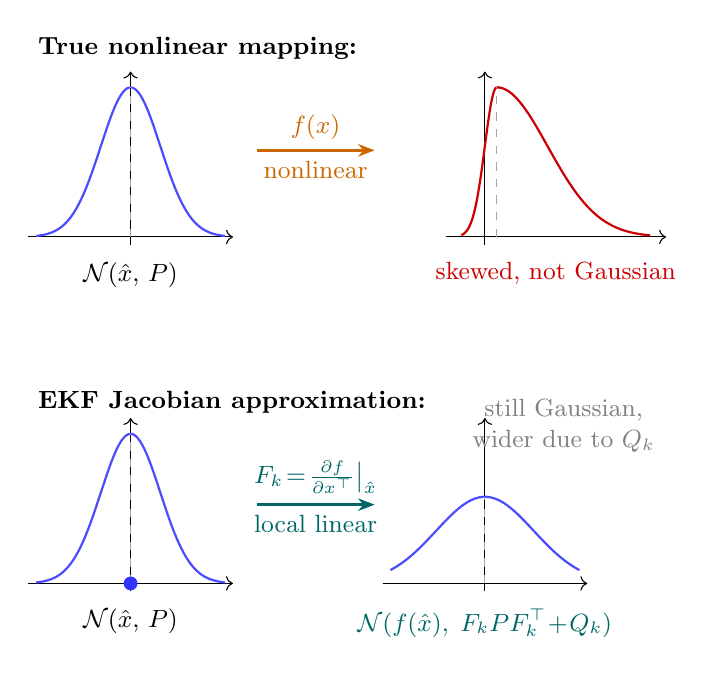
\begin{tikzpicture}[
      arr/.style={-{Stealth[length=6pt]}, very thick},
      lbl/.style={font=\small}
    ]

    % ══ ROW 1: nonlinear ══════════════════════════════════════════════════════
    \node[font=\bfseries\small, anchor=west] at (-1.3, 5.8)
      {True nonlinear mapping:};

    % Input Gaussian
    \begin{scope}[yshift=3.4cm]
      \draw[->] (-1.3,0) -- (1.3,0);
      \draw[->] (0,-0.1) -- (0,2.1);
      \draw[blue!70, thick, domain=-1.2:1.2, smooth, samples=50]
        plot (\x, {1.9*exp(-3.5*\x*\x)});
      \draw[dashed, gray!70] (0,0) -- (0,1.9);
      \node[lbl, below] at (0,-0.2) {$\mathcal{N}(\hat{x},\,P)$};
    \end{scope}

    % Arrow: nonlinear
    \draw[arr, orange!80!black] (1.6, 4.5) -- (3.1, 4.5)
      node[midway, above, lbl] {$f(x)$}
      node[midway, below, lbl, orange!80!black] {nonlinear};

    % Output: clearly skewed --- sharp left wall, long right tail
    \begin{scope}[xshift=4.5cm, yshift=3.4cm]
      \draw[->] (-0.5,0) -- (2.3,0);
      \draw[->] (0,-0.1) -- (0,2.1);
      \draw[red!80!black, thick, domain=-0.3:2.1, smooth, samples=100]
        plot (\x, {ifthenelse(\x < 0.15,
                    1.9*exp(-22*(\x-0.15)*(\x-0.15)),
                    1.9*exp(-1.2*(\x-0.15)*(\x-0.15)))});
      \draw[dashed, gray!70] (0.15,0) -- (0.15,1.9);
      \node[lbl, below, red!80!black] at (0.9,-0.2) {skewed, not Gaussian};
    \end{scope}

    % ══ ROW 2: Jacobian ═══════════════════════════════════════════════════════
    \node[font=\bfseries\small, anchor=west] at (-1.3, 1.3)
      {EKF Jacobian approximation:};

    % Input Gaussian
    \begin{scope}[yshift=-1.0cm]
      \draw[->] (-1.3,0) -- (1.3,0);
      \draw[->] (0,-0.1) -- (0,2.1);
      \draw[blue!70, thick, domain=-1.2:1.2, smooth, samples=50]
        plot (\x, {1.9*exp(-3.5*\x*\x)});
      \draw[dashed, gray!70] (0,0) -- (0,1.9);
      \fill[blue!80] (0,0) circle (2.5pt);
      \node[lbl, below] at (0,-0.2) {$\mathcal{N}(\hat{x},\,P)$};
    \end{scope}

    % Arrow: Jacobian
    \draw[arr, teal!80!black] (1.6, 0.0) -- (3.1, 0.0)
      node[midway, above, lbl, align=center]
        {$F_k\!=\!\tfrac{\partial f}{\partial x^\top}\big|_{\hat{x}}$}
      node[midway, below, lbl, teal!80!black] {local linear};

    % Output: symmetric, wider Gaussian
    \begin{scope}[xshift=4.5cm, yshift=-1.0cm]
      \draw[->] (-1.3,0) -- (1.3,0);
      \draw[->] (0,-0.1) -- (0,2.1);
      \draw[blue!70, thick, domain=-1.2:1.2, smooth, samples=50]
        plot (\x, {1.1*exp(-1.3*\x*\x)});
      \draw[dashed, gray!70] (0,0) -- (0,1.1);
      \node[lbl, below, teal!80!black, align=center] at (0,-0.2)
        {$\mathcal{N}(f(\hat{x}),\;F_k P F_k^\top\!+\!Q_k)$};
    \end{scope}

    % annotation
    \node[lbl, align=center, gray] at (5.5, 1.0)
      {still Gaussian,\\wider due to $Q_k$};

  \end{tikzpicture}
  \caption{Top: passing a Gaussian through a nonlinear $f$ produces a
           skewed, non-Gaussian output --- no simple covariance formula exists.
           Bottom: the EKF approximates $f$ as locally linear at $\hat{x}$
           using the Jacobian $F_k$, so the output remains Gaussian and
           the covariance can be propagated with $F_k P F_k^\top + Q_k$.
           The mean is simply evaluated: $f(\hat{x})$ gives the new centre
           directly.}
\end{figure}

\begin{keybox}
  \textbf{The EKF in one paragraph.}
  The filter tracks a Gaussian belief $\mathcal{N}(\hat{x}_k, P_k)$
  about the state.
  At each step, the \textbf{time update} predicts forward:
  the mean moves through the nonlinear $f$ directly
  ($\hat{x}_{k+1|k} = f(\hat{x}_{k|k}, u_k)$) while the covariance
  grows through the Jacobian $F_k$ plus process noise
  ($P_{k+1|k} = F_k P_{k|k} F_k^\top + Q_k$) --- uncertainty
  increases because the model is imperfect and the world is noisy.
  The \textbf{measurement update} then corrects both: the mean is
  nudged towards what the sensor said, and the covariance shrinks
  because a measurement is new information.
  The Jacobian $F_k$ is needed for the covariance because a Gaussian
  pushed through a nonlinear curve is no longer Gaussian --- the
  Jacobian linearises $f$ locally so the Gaussian-to-Gaussian
  propagation formula still applies.
  The mean can use $f$ directly because a point just needs to be
  evaluated, not transformed as a distribution.
\end{keybox}

% ==============================================================================
\section*{Section 3 \quad The Unscented Transform (UT)}
% ==============================================================================

% ------------------------------------------------------------------------------
\subsection*{Motivation: what problem does the UT solve?}
% ------------------------------------------------------------------------------

Both the EKF and UKF need to answer the same core question at every step:

\begin{center}
  \emph{Given a random variable $x$ with known mean $\mu_x$ and
  covariance $C_x$, what are the mean and covariance of
  $y = f(x)$ after passing through a nonlinear function $f$?}
\end{center}

For a \textbf{linear} $f$ this is easy --- matrices pass means and
covariances through exactly.
For a \textbf{nonlinear} $f$ there is no closed-form answer in general.
The EKF solves it by approximating $f$ as linear (Jacobian).
The UT takes a completely different approach: keep $f$ \emph{exact}
and instead choose a small, carefully placed set of sample points ---
called \textbf{sigma points} --- that capture the mean and covariance
of $x$, push each one through the actual nonlinear $f$, and estimate
the output statistics from the results.

% ------------------------------------------------------------------------------
\subsection*{Three approaches compared}
% ------------------------------------------------------------------------------

\begin{figure}[H]
  \centering
  
\includegraphics[width=0.92\textwidth]{slide-17.jpg}
  \caption{The generic probabilistic problem and the linearisation
           (EKF) solution.}
\end{figure}

\begin{center}
\renewcommand{\arraystretch}{1.5}
\begin{tabular}{p{2.5cm} p{4cm} p{6.5cm}}
  \toprule
  \textbf{Method} & \textbf{How it works} & \textbf{Key point} \\
  \midrule
  Linearisation (EKF) &
    Replace $f$ with its tangent (Jacobian) at $\mu_x$. &
    Fast, but introduces error wherever $f$ curves. \\
  Monte Carlo (MC) &
    Draw thousands of random samples $x_i$, compute $f(x_i)$
    for each, estimate mean and covariance from the sample. &
    Accurate but needs very many samples --- expensive. \\
  Unscented Transform &
    Choose $2n+1$ deterministic sigma points that exactly
    represent $\mu_x$ and $C_x$, push each through $f$,
    form weighted mean and covariance of the outputs. &
    No Jacobians, uses actual $f$, needs only $2n+1$ points. \\
  \bottomrule
\end{tabular}
\end{center}

\begin{notebox}
  The UT is essentially Monte Carlo, but the samples are
  \textbf{not random} --- they are constructed deterministically
  to encode exactly the right mean and covariance.
  Because they are chosen optimally, only $2n+1$ points are needed
  (where $n$ is the state dimension) instead of the thousands
  required by MC.
\end{notebox}

% ------------------------------------------------------------------------------
\subsection*{UT algorithm: sigma points and weights}
% ------------------------------------------------------------------------------

\begin{figure}[H]
  \centering
  
\includegraphics[width=0.92\textwidth]{slide-19.jpg}
  \caption{The full UT algorithm.}
\end{figure}

\textbf{Step 1 --- Parameters} (default values $\alpha=1$,
$\kappa=2$, $\beta=0$ give $\lambda = 2$):
\[
  \lambda = \alpha^2(n+\kappa) - n, \qquad
  k = \sqrt{n+\lambda}, \qquad
  n = \dim(x)
\]

$\lambda$ is a scaling parameter controlling how far the sigma points
are spread from the mean. $k$ is the actual distance multiplier used
when placing them. With the default values and $n=2$ states:
$\lambda = 1^2(2+2)-2 = 2$, $k = \sqrt{2+2} = 2$.
The larger $n$ is, the further out the points are placed to
cover the wider spread of a higher-dimensional Gaussian.

\textbf{Step 2 --- Sigma points} (eigenvalue decomposition version).
The covariance matrix $C_x$ is decomposed into its eigenvectors $u_i$
and eigenvalues $l_i$ --- this is called the \textbf{eigenvalue
decomposition} (also called spectral decomposition).
Let $u_i$ be the $i$-th eigenvector and $l_i$ the $i$-th eigenvalue
of $C_x$.
The $2n+1$ sigma points are:
\[
  x_i = \begin{cases}
    \mu_x & i = 0 \\
    \mu_x + k\,u_i\sqrt{l_i} & 1 \leq i \leq n \\
    \mu_x - k\,u_i\sqrt{l_i} & n+1 \leq i \leq 2n
  \end{cases}
\]

\begin{notebox}
  \textbf{What are the sigma points --- concretely?}\\
  Say you have a 2D state ($n=2$), so $2n+1 = 5$ sigma points total:
  \begin{itemize}[leftmargin=1.4em, topsep=2pt]
    \item $x_0 = \mu_x$ \hfill --- the mean itself, one point at the centre
    \item $x_1 = \mu_x + k\,u_1\sqrt{l_1}$ \hfill --- pushed out along
          the first principal axis of the covariance ellipse
    \item $x_2 = \mu_x + k\,u_2\sqrt{l_2}$ \hfill --- pushed out along
          the second principal axis
    \item $x_3 = \mu_x - k\,u_1\sqrt{l_1}$ \hfill --- mirror of $x_1$
    \item $x_4 = \mu_x - k\,u_2\sqrt{l_2}$ \hfill --- mirror of $x_2$
  \end{itemize}
  The eigenvectors $u_i$ point along the axes of the covariance ellipse
  (the directions of greatest and least uncertainty).
  The eigenvalues $l_i$ give the variance in each direction --- so
  $\sqrt{l_i}$ is roughly the standard deviation.
  Multiplying by $k$ controls how many standard deviations out
  the points sit.
  Together these five points encode exactly the same mean and
  covariance as the original Gaussian --- no random sampling needed.
\end{notebox}

\textbf{Step 3 --- Weights.}
Each sigma point gets a weight for computing the output mean ($w^m$)
and a separate weight for computing the output covariance ($w^c$).
The centre point $x_0$ gets a different weight from the others because
it sits at the mean and carries more representative information:
\[
  w_i^m = \begin{cases}
    \dfrac{\lambda}{n+\lambda} & i = 0 \\[6pt]
    \dfrac{1}{2(n+\lambda)} & 1 \leq i \leq 2n
  \end{cases}
  \qquad
  w_i^c = \begin{cases}
    \dfrac{\lambda}{n+\lambda} + 1 - \alpha^2 + \beta & i = 0 \\[6pt]
    \dfrac{1}{2(n+\lambda)} & 1 \leq i \leq 2n
  \end{cases}
\]

\begin{notebox}
  \textbf{Weights: what they are and when they change.}\\[4pt]
  \textbf{Are the weights fixed?}
  Yes --- once you choose $\alpha$, $\kappa$, $\beta$ and know $n$
  (the state dimension), all weights are computed once and stay
  constant for every step of the filter.
  They do not depend on the current state estimate or covariance.\\[4pt]
  \textbf{Why two sets?}
  $w_i^m$ controls how much each mapped sigma point contributes to
  the \emph{output mean} estimate.
  $w_i^c$ controls how much each contributes to the
  \emph{output covariance} estimate.
  For the outer points ($i \geq 1$) the two weights are identical.
  Only the centre point $i=0$ differs, because the extra term
  $1 - \alpha^2 + \beta$ allows tuning how much the centre point
  influences the covariance independently of the mean.\\[4pt]
  \textbf{Numerical example with default values ($n=2$,
  $\alpha=1$, $\kappa=2$, $\beta=0$, so $\lambda=2$):}
  \begin{itemize}[leftmargin=1.4em, topsep=2pt]
    \item \textit{Mean weights}:
          $w_0^m = \dfrac{\lambda}{n+\lambda} = \dfrac{2}{4} = 0.5$,
          \quad $w_{1\ldots4}^m = \dfrac{1}{2(n+\lambda)} = \dfrac{1}{8} = 0.125$\\
          Check: $0.5 + 4\times 0.125 = 1$ \checkmark
    \item \textit{Covariance weights}:
          $w_0^c = \dfrac{\lambda}{n+\lambda} + 1 - \alpha^2 + \beta
          = 0.5 + 1 - 1 + 0 = 0.5$,
          \quad $w_{1\ldots4}^c = 0.125$\\
          Check: $0.5 + 4\times 0.125 = 1$ \checkmark
  \end{itemize}
  With default $\beta=0$ and $\alpha=1$, the extra term is zero so
  $w_0^c = w_0^m$ --- the centre point has the same influence on both
  mean and covariance.
  Setting $\beta=2$ (optimal for a Gaussian input) gives
  $w_0^c = 0.5 + 1 - 1 + 2 = 2.5$ --- the centre point gets much
  more weight for covariance, which improves accuracy when the input
  really is Gaussian.
  The outer weights stay at $0.125$ regardless.
\end{notebox}

\textbf{Step 4 --- Propagate and compute output statistics.}
Push each sigma point through the actual nonlinear $f$
(no Jacobian, no approximation), then form weighted sums:

\medskip
\textit{Output mean} --- weighted average of where the sigma points
land after $f$:
\[
  \hat{\mu}_y = \sum_{i=0}^{2n} w_i^m\, f(x_i)
\]

\textit{Output cross-covariance} --- weighted measure of how much
the output $f(x_i)$ and the input $x_i$ move together
(needed for the Kalman gain in the UKF):
\[
  \hat{C}_{yx} = \sum_{i=0}^{2n} w_i^c\,
    \bigl(f(x_i) - \hat{\mu}_y\bigr)(x_i - \mu_x)^\top
\]

\textit{Output covariance} --- weighted spread of the mapped sigma
points around the estimated output mean:
\[
  \hat{C}_y = \sum_{i=0}^{2n} w_i^c\,
    \bigl(f(x_i) - \hat{\mu}_y\bigr)\bigl(f(x_i) - \hat{\mu}_y\bigr)^\top
\]

\begin{notebox}
  \textbf{What do these three output quantities give you?}
  \begin{itemize}[leftmargin=1.4em, topsep=2pt]
    \item $\hat{\mu}_y$ --- estimated mean of $y = f(x)$
          (weighted average of where the sigma points land after $f$).
    \item $\hat{C}_y$ --- estimated covariance of $y$
          (weighted spread of the mapped sigma points around $\hat{\mu}_y$).
    \item $\hat{C}_{yx}$ --- estimated cross-covariance between $y$
          and $x$ (how much they move together) ---
          this is needed for the Kalman gain in the UKF.
  \end{itemize}
\end{notebox}

% ------------------------------------------------------------------------------
\subsection*{Important properties of the UT}
% ------------------------------------------------------------------------------

\begin{keybox}
  \begin{itemize}[leftmargin=1.4em, topsep=2pt]
    \item \textbf{Exact for affine functions.}
          If $f(x) = Ax + b$ (linear plus offset), the UT gives the
          exact mean and covariance --- same as the standard KF would.
          This is a consistency check: the UT should at least match
          the KF when the system is actually linear.
    \item \textbf{Good approximation for nonlinear $f$.}
          The UT captures the mean and covariance correctly to
          second order in a Taylor expansion, whereas the EKF
          (linearisation) is only accurate to first order.
          This means the UT is generally \textbf{more accurate}
          than the EKF, especially for highly nonlinear systems.
    \item \textbf{No Jacobians needed.}
          $f$ is used as a black box --- you never compute
          $\partial f / \partial x$.
          This is a major practical advantage when $f$ is
          complicated or the derivative is hard to derive.
    \item \textbf{Generally superior to both linearisation and MC.}
          Better accuracy than EKF with far fewer evaluations of
          $f$ than MC ($2n+1$ vs thousands).
  \end{itemize}
\end{keybox}

% ------------------------------------------------------------------------------
\subsection*{Example and comparison plots}
% ------------------------------------------------------------------------------

The test case uses $y = x^\top x$ with $x \in \mathbb{R}^2$ ---
a 2D state with $E(x) = [1,\,1]^\top$ and
$\mathrm{Cov}(x) = \bigl[\begin{smallmatrix}1&1\\1&2\end{smallmatrix}\bigr]$.
The function $y = x^\top x = x_1^2 + x_2^2$ is a scalar output ---
the squared distance from the origin.
It is nonlinear (involves products of states), so the output
distribution is not Gaussian.
The correct answer is known analytically, so errors can be measured.

\begin{figure}[H]
  \centering
  
\includegraphics[width=0.88\textwidth]{slide-21.jpg}
  \caption{UT: sigma points in input space (top) and their mapped
           values in output space (bottom). $n=2$ states so
           $2n+1=5$ sigma points total.
           \textbf{Top plot} --- axes are $x_1$ and $x_2$ (the two
           state components). The 5 sigma points are shown as $+$
           marks: one at the mean $[1,1]^\top$ and four pushed out
           symmetrically along the principal axes of the covariance
           ellipse.
           \textbf{Bottom plot} --- each sigma point has been put
           through $f$, giving a scalar $y_i = x_{i,1}^2 + x_{i,2}^2$.
           The 5 output values are shown on the $y$-axis as $+$ marks.
           The weighted mean and variance of these 5 numbers gives the
           UT estimate of the output distribution.}
\end{figure}

\begin{figure}[H]
  \centering
  
\includegraphics[width=0.88\textwidth]{slide-22.jpg}
  \caption{MC comparison using thousands of random samples.
           \textbf{Top plot} --- axes are again $x_1$ and $x_2$.
           Instead of 5 chosen points, thousands of random samples
           are drawn from $\mathcal{N}([1,1]^\top, C_x)$ --- the
           dense blue cloud.
           \textbf{Bottom plot} --- every sample is put through $f$,
           giving a cloud of scalar $y$ values along the axis.
           The sample mean and variance of this cloud estimates the
           output statistics.
           The UT (5 points) achieves essentially the same answer
           as MC (thousands of points).}
\end{figure}

\begin{figure}[H]
  \centering
  
\includegraphics[width=0.88\textwidth]{slide-23.jpg}
  \caption{Comparison of sigma point placement:
           \textbf{eigenvalue decomposition} (blue $+$, the version
           used in the algorithm above) vs.\
           \textbf{Cholesky decomposition} (green $\circ$, an
           alternative).
           Both place points along the principal directions of the
           covariance ellipse, but they arrive at those directions
           differently.
           The eigenvalue method decomposes $C_x$ into eigenvectors
           and eigenvalues directly.
           The Cholesky method instead factors $C_x = LL^\top$
           (where $L$ is a lower-triangular matrix) and uses the
           columns of $L$ to place the points --- no eigenvectors
           needed, which is faster to compute.
           Both give valid sigma points and the same final estimates;
           Cholesky is the more common choice in practice for
           this reason.}
\end{figure}

\begin{figure}[H]
  \centering
  
\includegraphics[width=0.88\textwidth]{slide-24.jpg}
  \caption{Performance comparison table for the test case
           $y = x^\top x$, $x \in \mathbb{R}^2$.}
\end{figure}

\begin{notebox}
  \textbf{Reading the performance table.}\\[4pt]
  \textbf{Columns} --- the four output quantities being estimated:
  \begin{itemize}[leftmargin=1.4em, topsep=2pt]
    \item $M_y$ --- the estimated \textbf{mean} of the output $y$.
          Correct answer: $E[y] = E[x_1^2 + x_2^2] = 5$.
    \item $C_y$ --- the estimated \textbf{variance} of $y$
          (since $y$ is a scalar, this is a single number).
          Correct answer: $34$.
    \item $C_{yx}$ (two numbers) --- the estimated
          \textbf{cross-covariance} between $y$ and each component of
          $x$: how much does $y$ move when $x_1$ moves, and how much
          when $x_2$ moves.
          Correct answer: $[4,\; 6]$.
  \end{itemize}

  \textbf{Rows} --- the four methods being compared:
  \begin{itemize}[leftmargin=1.4em, topsep=2pt]
    \item \textbf{UTSCEst} --- UT using Cholesky decomposition
          (the green $\circ$ points from the previous figure).
    \item \textbf{UTJMEst} --- UT using eigenvalue decomposition
          (the blue $+$ points; the version in the algorithm above).
    \item \textbf{MCEst} --- Monte Carlo estimate using thousands
          of random samples.
    \item \textbf{THTK} --- the theoretical correct answer, computed
          analytically.
          This is the target every method is trying to hit.
  \end{itemize}

  \textbf{RelE rows} --- relative error of each method compared to
  THTK, i.e.\ $(\text{estimate} - \text{correct})/\text{correct}$.
  Zero means perfect.\\[4pt]

  \textbf{What to take away:}
  \begin{itemize}[leftmargin=1.4em, topsep=2pt]
    \item Both UT methods get $M_y$ and $C_{yx}$ \textbf{exactly right}
          (RelE $= 0$) --- the mean and cross-covariance are perfect.
    \item There is a small error in $C_y$ (the variance) --- around
          15\% for UTSC and $-9\%$ for UTJM.
          This is expected: the UT is not exact for nonlinear $f$,
          but it is a good approximation.
    \item MC has small errors \emph{everywhere} ($< 1\%$) because it
          uses very many samples, but it achieves this at the cost of
          thousands of function evaluations versus just 5 for the UT.
  \end{itemize}
\end{notebox}

% ==============================================================================
\section*{Section 4 \quad The Unscented Kalman Filter (UKF)}
% ==============================================================================

% ------------------------------------------------------------------------------
\subsection*{From UT to UKF: the key idea}
% ------------------------------------------------------------------------------

The UT solves the core problem of propagating a mean and covariance
through a nonlinear function.
The UKF simply \textbf{plugs the UT into the general KF equations}
wherever a nonlinear propagation is needed --- once for the
measurement function $h$ (Step B) and once for the state function $f$
(Step A).
No Jacobians anywhere.

To keep the notation compact, the UT is written as a single function
$U$:
\[
  \begin{bmatrix} E(y) \\ \mathrm{Cov}(y,x) \\ \mathrm{Cov}(y) \end{bmatrix}
  = U\!\left(f,\; E(x),\; \mathrm{Cov}(x)\right)
\]

In words: give $U$ the function, the current mean, and the current
covariance --- it runs the sigma-point machinery internally and
returns the output mean, the output covariance, and the
cross-covariance.

The same formula works when everything is \textbf{conditioned on
some known information $z$}:
\[
  \begin{bmatrix} E(y \mid z) \\ \mathrm{Cov}(y,x \mid z) \\ \mathrm{Cov}(y \mid z) \end{bmatrix}
  = U\!\left(f,\; E(x \mid z),\; \mathrm{Cov}(x \mid z)\right)
\]

\begin{notebox}
  \textbf{What does ``conditioned on $z$'' mean?}\\
  Conditioning on $z$ just means: \emph{given that we already know
  $z$}, what are the statistics?
  If $z = \mathcal{Y}_{k-1}$ (all measurements up to step $k-1$),
  then $E(x \mid z) = \hat{x}_{k|k-1}$ is our estimated mean
  \emph{taking all past measurements into account}, and
  $\mathrm{Cov}(x \mid z) = P_{k|k-1}$ is our uncertainty given
  that same information.\\[4pt]
  The point of writing it this way is to show that the UT works
  identically whether the inputs are raw (no prior information) or
  conditional on past data --- you just feed in whatever mean and
  covariance you currently have, and the UT gives back the
  corresponding output statistics.
  In the KF, $z$ is always the set of past measurements
  $\mathcal{Y}_{k-1}$, so the outputs are automatically conditioned
  on everything we have seen so far.
\end{notebox}

\begin{figure}[H]
  \centering
  
\includegraphics[width=0.85\textwidth]{slide-25.jpg}
  \caption{UKF definition: the UT written as a compact function $U$.}
\end{figure}

% ------------------------------------------------------------------------------
\subsection*{UKF algorithm}
% ------------------------------------------------------------------------------

The structure mirrors the EKF exactly --- same two-step predict and
correct --- but every place the EKF used a Jacobian, the UKF calls
$U$ instead.

\textbf{Initial conditions:}
\[
  x_0 \sim \mathcal{N}(\hat{x}_{0|-1},\; P_{0|-1})
\]

\textbf{Step B --- Measurement update} (after receiving $y_k$ and $u_k$):

First, run the UT on the measurement function $h$ to get the
predicted measurement, its covariance, and the cross-covariance
with the state:
\[
  \begin{bmatrix} \hat{y}_{k|k-1} \\ \mathrm{Cov}(y_k, x_k \mid \mathcal{Y}_{k-1}) \\ C_k^h \end{bmatrix}
  = U\!\left(h,\; \hat{x}_{k|k-1},\; P_{k|k-1}\right)
\]

\textbf{(1) Total measurement uncertainty} --- the UT gave us $C_k^h$,
the covariance of the predicted measurement due to state uncertainty.
But the sensor itself also has noise $R_k$.
Add them together to get the full uncertainty in what the sensor reads:
\[
  \mathrm{Cov}(y_k \mid \mathcal{Y}_{k-1}) = C_k^h + R_k
\]

\textbf{(2) Innovation} --- compare what the sensor actually read
($y_k$) to what the UT predicted it would read ($\hat{y}_{k|k-1}$).
The difference is how wrong the prediction was:
\[
  \tilde{y}_{k|k-1} = y_k - \hat{y}_{k|k-1}
\]

\textbf{(3) Kalman gain} --- how much should we trust the innovation?
The cross-covariance $\mathrm{Cov}(x_k, y_k)$ (from the UT) tells us
how strongly the state and measurement are linked.
Dividing by the total measurement uncertainty scales the correction:
large sensor noise $\Rightarrow$ small $K_k$ $\Rightarrow$ small
correction; precise sensor $\Rightarrow$ large $K_k$ $\Rightarrow$
big correction:
\[
  K_k = \mathrm{Cov}(x_k, y_k \mid \mathcal{Y}_{k-1})\;
        \mathrm{Cov}(y_k \mid \mathcal{Y}_{k-1})^{-1}
\]

\textbf{(4) State mean update} --- nudge the predicted state estimate
in the direction the innovation says we were wrong, scaled by $K_k$:
\[
  \hat{x}_{k|k} = \hat{x}_{k|k-1} + K_k\,\tilde{y}_{k|k-1}
\]

\textbf{(5) Covariance update} --- the measurement gave us new
information, so uncertainty shrinks.
How much it shrinks depends on how strongly the state and measurement
are linked (the cross-covariance from the UT):
\[
  P_{k|k} = P_{k|k-1} - K_k\,\mathrm{Cov}(y_k, x_k \mid \mathcal{Y}_{k-1})
\]

\begin{figure}[H]
  \centering
  
\includegraphics[width=0.85\textwidth]{slide-26.jpg}
  \caption{UKF algorithm --- measurement update.}
\end{figure}

\textbf{Step A --- Time update} (propagate from $k$ to $k+1$):

\textbf{(1) Run the UT on $f$} --- feed the current updated estimate
$\hat{x}_{k|k}$ and covariance $P_{k|k}$ into the UT together with
the state function $f$.
The UT places sigma points around $\hat{x}_{k|k}$, pushes each one
through the actual nonlinear $f$, and returns three things: the
predicted next state mean, the unused cross-covariance $X$, and
$C_k^f$ (the covariance of the predicted next state due to state
uncertainty alone --- process noise not yet included):
\[
  \begin{bmatrix} \hat{x}_{k+1|k} \\ X \\ C_k^f \end{bmatrix}
  = U\!\left(f,\; \hat{x}_{k|k},\; P_{k|k}\right)
\]

\textbf{(2) Add process noise} --- $C_k^f$ only accounts for how the
current uncertainty in $x_k$ spreads through $f$.
It does not yet include the random disturbances that hit the system
between steps ($w_k \sim \mathrm{NID}(0, Q_k)$).
Adding $Q_k$ gives the full predicted covariance for the next step:
\[
  P_{k+1|k} = C_k^f + Q_k
\]

\begin{figure}[H]
  \centering
  
\includegraphics[width=0.85\textwidth]{slide-27.jpg}
  \caption{UKF algorithm --- time update.}
\end{figure}

\begin{notebox}
  \textbf{What is $X$ in the time update?}\\
  $X$ is the cross-covariance $\mathrm{Cov}(x_{k+1}, x_k \mid \mathcal{Y}_k)$
  --- how much the next state and the current state move together.
  It is an output of $U$ but is \textbf{not used} in the standard UKF
  time update equations; only $\hat{x}_{k+1|k}$ and $C_k^f$ are needed.
  It would only matter in more advanced formulations.
\end{notebox}

% ------------------------------------------------------------------------------
\subsection*{EKF vs UKF side by side}
% ------------------------------------------------------------------------------

The $\dagger$ symbol marks quantities that come directly out of the
UT call $U$ --- no extra computation needed.

\begin{center}
\renewcommand{\arraystretch}{1.8}
\begin{tabular}{p{2.8cm} p{5.0cm} p{5.0cm}}
  \toprule
  & \textbf{EKF} & \textbf{UKF} \\
  \midrule
  Mean update (B) &
    $\hat{y}_{k|k-1} = h(\hat{x}_{k|k-1}, u_k)$\newline
    {\footnotesize single point evaluation of $h$} &
    $\hat{y}_{k|k-1}^\dagger$ from $U(h, \hat{x}_{k|k-1}, P_{k|k-1})$\newline
    {\footnotesize weighted mean of sigma points through $h$} \\
  Cov.\ update (B) &
    $(I{-}K_k H_k)P(I{-}K_k H_k)^\top$\newline${+}K_k R_k K_k^\top$\newline
    {\footnotesize $H_k$ = Jacobian of $h$} &
    $P_{k|k-1} - K_k \mathrm{Cov}(y_k, x_k)^\dagger$\newline
    {\footnotesize $\mathrm{Cov}(y_k, x_k)$ from $U$, no Jacobian} \\
  Gain $K_k$ &
    $P_{k|k-1} H_k^\top (H_k P_{k|k-1} H_k^\top + R_k)^{-1}$\newline
    {\footnotesize built from Jacobian $H_k$} &
    $\mathrm{Cov}(x_k, y_k)^\dagger\,\mathrm{Cov}(y_k)^{-1}$\newline
    {\footnotesize both covariances come from $U$ directly} \\
  Mean update (A) &
    $\hat{x}_{k+1|k} = f(\hat{x}_{k|k}, u_k)$\newline
    {\footnotesize single point evaluation of $f$} &
    $\hat{x}_{k+1|k}^\dagger$ from $U(f, \hat{x}_{k|k}, P_{k|k})$\newline
    {\footnotesize weighted mean of sigma points through $f$} \\
  Cov.\ update (A) &
    $F_k P_{k|k} F_k^\top + Q_k$\newline
    {\footnotesize $F_k$ = Jacobian of $f$} &
    $C_k^{f\,\dagger} + Q_k$\newline
    {\footnotesize $C_k^f$ from $U$, $Q_k$ added for process noise} \\
  Jacobians? &
    Yes --- $F_k$ and $H_k$ every step &
    No --- $f$ and $h$ are black boxes \\
  Optimal? & No & No \\
  Stable? & Not guaranteed & Not guaranteed \\
  \bottomrule
\end{tabular}
\end{center}

\begin{keybox}
  \textbf{Key takeaways --- Section 4}
  \begin{itemize}[leftmargin=1.4em, topsep=2pt]
    \item The UKF replaces \textbf{both} the mean update and the
          covariance update with a single call to $U$.
          In the EKF these are two separate jobs: evaluate $f$ or $h$
          at one point for the mean, then use the Jacobian for the
          covariance.
          In the UKF, one UT call handles both at once --- push
          $2n+1$ sigma points through the actual $f$ or $h$, and
          you immediately get the output mean, output covariance,
          and cross-covariance all together.
    \item The structure is identical to the EKF:
          two steps, same gain formula, same correction logic.
          Only the \emph{mechanism} for computing means and covariances
          is different.
    \item The UKF Kalman gain uses $\mathrm{Cov}(x_k, y_k)$ and
          $\mathrm{Cov}(y_k)$ directly --- these come out of the UT
          automatically, no matrix inversion of a Jacobian needed.
    \item Like the EKF, the UKF is \textbf{not optimal} and
          \textbf{not guaranteed stable}.
  \end{itemize}
\end{keybox}

\begin{notebox}
  \textbf{Why the UKF is more accurate than the EKF --- Taylor
  expansion argument.}\\[6pt]

  \textbf{Why the EKF is only first-order accurate.}\\
  The EKF linearises $f$ by truncating the Taylor expansion after
  the first term:
  \[
    f(x) \approx f(\hat{x}) + \underbrace{F_k}_{\text{1st derivative}}(x - \hat{x})
  \]
  The next term in the series would be
  $\frac{1}{2}(x-\hat{x})^\top H_f (x-\hat{x})$
  where $H_f$ is the \textbf{Hessian} --- the matrix of second
  derivatives describing the curvature of $f$.
  The EKF throws this away entirely.
  Any effect the curvature has on the mean or covariance is simply
  missed. That is what first-order accurate means: only the first
  derivative is used, everything else is ignored.\\[6pt]

  \textbf{Why the UT is second-order accurate for any distribution.}\\
  $\delta$ is the offset from the mean to one sigma point --- the
  direction and distance you push out.
  The UT evaluates $f$ at two symmetric points: one step forward
  from the mean, one step backward.
  Taylor-expand each:
  \begin{align*}
    f(\hat{x}+\delta) &\approx f(\hat{x}) + F\cdot\delta
      + \tfrac{1}{2}\,\delta^\top H_f\,\delta \\
    f(\hat{x}-\delta) &\approx f(\hat{x}) - F\cdot\delta
      + \tfrac{1}{2}\,\delta^\top H_f\,\delta
  \end{align*}
  Now add them:
  \[
    f(\hat{x}+\delta) + f(\hat{x}-\delta)
    \approx 2f(\hat{x}) + \underbrace{\delta^\top H_f\,\delta}_{\text{2nd order term}}
  \]
  The first-order terms $+F\cdot\delta$ and $-F\cdot\delta$
  \textbf{cancel} because the points are symmetric.
  What survives is $2f(\hat{x})$ (twice the value at the mean)
  plus the curvature term $\delta^\top H_f\,\delta$.
  Dividing by 2 and weighting gives $f(\hat{x})$ plus a correction
  for how curved $f$ is in direction $\delta$ --- without ever
  computing $H_f$ explicitly.
  The sigma points capture the second-order term automatically just
  by being symmetric.
  This is why the UT is \textbf{second-order accurate for any input
  distribution}.\\[6pt]

  \textbf{Why it is third-order accurate for Gaussian inputs.}\\
  A Gaussian distribution is perfectly symmetric, so all its
  \emph{odd} moments are zero --- there is no skew.
  The third-order error term in the Taylor expansion involves the
  third moment of $(x-\hat{x})$.
  For a Gaussian that moment is exactly zero, so the third-order
  error vanishes automatically.
  The UT therefore achieves \textbf{third-order accuracy} when the
  input is Gaussian, at no extra cost.\\[6pt]

  \begin{center}
  \renewcommand{\arraystretch}{1.4}
  \begin{tabular}{p{2.2cm} p{2.5cm} p{7.5cm}}
    \toprule
    \textbf{Method} & \textbf{Accuracy} & \textbf{Why} \\
    \midrule
    EKF &
      1st order &
      Uses only Jacobian (first derivative); Hessian/curvature
      thrown away \\
    UKF &
      2nd order\newline(any input) &
      Symmetric sigma points cause first-order terms to cancel;
      second-order curvature captured automatically \\
    UKF &
      3rd order\newline(Gaussian input) &
      Odd moments of a Gaussian are zero, so the third-order
      error term vanishes \\
    \bottomrule
  \end{tabular}
  \end{center}
\end{notebox}

\end{document}
